\chapter{Marco Teórico}

El marco teórico del proyecto se limita al estudio de la naturaleza de las comunicaciones usadas. El trabajo emplea dos tipos de comunicaciones: raciofrecuencia y serial. La radiofrecuencia es la comunicación usada entre los módulos XBee. Por otro lado, la comunicación entre los módulos mencionados y sus correspondientes dispositivos de control se realiza por método serial. A continuación se comentan los conceptos básicos para comprender ambos métodos de comunicación.

\section{Conceptos de la comunicación serial}

La comunicación serie (o serial) es un método de transmisión de datos consistente en el envío de un único bit en un mismo instante de forma secuencial por una simple línea de transmisión. Lo simple de este método ha hecho que la comunicación serial se extienda masivamente entre los dispositivos comerciales, siendo actualmente un método común para comunicar ordenadores con distintos periféricos.

Se opone a la llamada comunicación paralela, que precisa de una línea de transmisión por cada bit de datos a cambio de un aumento de las prestaciones. Es bastante usual usar ocho líneas de datos, correspondiente a un byte. El uso de un número elevado de líneas de datos además de las líneas de control, hace notablemente mas caro el uso de comunicación paralela. Sumado a esto, la comunicación serie se ha desarrollado bajo un marco de estandarización mucho más extendido que en la comunicación paralela \cite{DispLogicos}; yendo esta característica en contra de implantar sistemas paralelos.

\subsection{Características}

Los bits secuenciales son transmitidos a partir del uso de dos niveles lógicos que pueden ser de tensión (más usual) o de corriente. Estos niveles se corresponden en el llamado \textit{formato marca espacio} (figura \ref{fig:marcaespacio}) con los niveles lógicos "0" y "1". Al nivel lógico "0" se le denomina espacio mientras que al nivel lógico "1" se le llama marca.

\begin{figure}[tb]
\centering
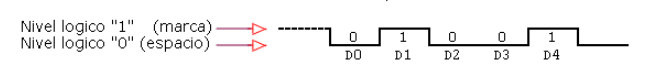
\includegraphics[width=0.75\textwidth]{figuras/marcaespacio.png}
\caption{Formato serie marca/espacio}
\label{fig:marcaespacio}
\end{figure}

Existen varias configuraciones de las lineas de comunicación \cite{DispLogicos}, cada uno optimiza sus prestaciones en relación a los requerimientos de la aplicación.
\begin{itemize}
\item La configuración \textit{simplex} únicamente precisa de un hilo de comunicación y, pese a su ligero menor coste de producción, no es muy usado debido a sus limitaciones. Estas limitaciones son, en primer lugar, la escasa flexibilidad resultado de la necesidad de establecer una relación emisor-receptor permanente; es decir, uno de los dispositivos será siempre emisor y el otro será siempre receptor. Por otro lado, no se permite la comprobación de la recepción de la informacion, posibilitando comunicaciones deficientes.
\item La configuración \textit{semi duplex} utiliza igualmente una línea de comunicación pero conmutando la etiqueta de emisor y receptor entre los dispositivos de manera periódica. Uno de los dispositivos emite la información para pasar a recibirla a continuación. Esto soluciona los problemas de la configuración \textit{simplex}, permitiendo hacer una comprobación de errores en la transmisión de datos.
\item La mayoría de casos de uso de la comunicación serie emplean la configuración \textit{full duplex} que permite la transmisión y recepción simultánea de datos por parte de ambos dispositivos. Para ello, se hace uso de dos líneas de comunicación, una destinada a la transmisión y otra a la recepción.
\end{itemize}

La base del funcionamiento de la comunicación es la sincronización. Para resolver esta cuestión en el caso de la comunicación serie, se estandarizan varios bits (o series de bits) y parametros entre emisor y receptor con el fin de determinar cuál es la información.

Existen dos modos de transmisión:
\begin{itemize}
\item El modo \textbf{síncorno} no usa bits de sincornización y todos los componentes de la transmisión se agrupan en bloques consecutivos, existiendo una secuencia de sincronización al inicio de cada bloque. El emisor indica al receptor que se va a iniciar una comunicación mediante el envío de un octeto de bits \textit{"sync"} (figura \ref{fig:serialsincrono}).

\begin{figure}[H]
\centering
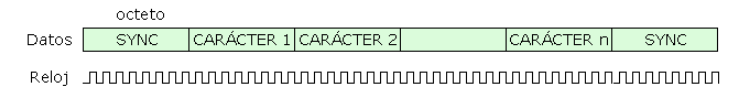
\includegraphics[width=0.75\textwidth]{figuras/SerialSincrono.png}
\caption{Transmisión serial síncrona}
\label{fig:serialsincrono}
\end{figure}

\item Por otro lado, el modo \textbf{asíncrono} no utiliza una línea de reloj, por lo que deben coincidir las características de la comunicación, como la velocidad de transmisión de datos, entre los dispositivos conectados. Para conseguir la sincronización en la comunicación, se hace uso de, por ejemplo, bits de inicio o parada (figura \ref{fig:serialasincrono}). Hay que tener en cuenta que la frecuencia a la que estos dispositivos leen el estado del frame es mucho mayor que la frecuencia a la que cambian de estado los propios bits del frame. En las siguientes líneas se definen conceptos relacionados con este tipo de comunicación, que es la utilizada a lo largo del proyecto.
\end{itemize}

La indicación del inicio de la comunicación del frame transmitido se realiza mediante el \textbf{start bit}. Este bit genera un flanco negativo (transición de nivel marca a nivel espacio) cuando la linea de datos está a nivel marca ("1" lógico) mientras no se transmita información (figura \ref{fig:serialasincrono}).

\begin{figure}[tb]
\centering
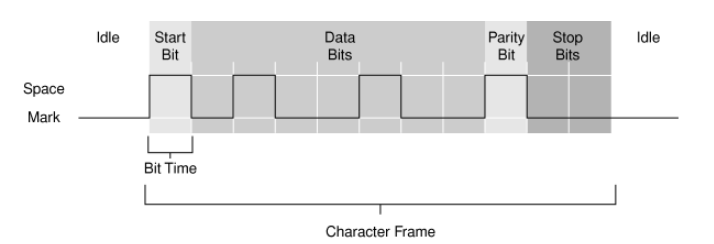
\includegraphics[width=0.75\textwidth]{figuras/SerialAsincrono.png}
\caption{Transmisión serial asíncrona}
\label{fig:serialasincrono}
\end{figure}

Existen varios parámetros que especifican y definen la comunicación serial \cite{NI:2004}, y que deberán ser comunes entre los dispositivos partícipes de la transmisión de datos. A continuación se enumeran los principales parámetros configurables. Una diferencia en la configuración de los dispositivos impedirá su comunicación.

\begin{itemize}
\item La llamada \textbf{Baud rate} o, en castellano, tasa de baudios, se trata de la cuantificación de las símbolos por segundo de una comunicación y sirve para medir la velocidad de transmisión de la información.Coincide con los bits por segundo siempre que un símbolo de transmisión contenga un bit. Sin embargo, esto no tiene porqué cumplirse y el número de bits transmitidos por segundo pueden ser mayores que los baudios. La velocidad de transmisión se limita con el ancho de banda y la potencia de la señal.
\item El número de \textbf{bits de datos} que se precisan para codificar un símbolo de información transmitido. Se suele tender a estandarizar el número de bits entre 5 y 8 bits. 
\item El \textbf{Parity bit} es opcional y se usa para la detección de errores. Se incrusta en medio del frame de bits de tal modo que es comprobable la correcta recepción del mismo. Se puede configurar como un bit de paridad par o impar. En el primer caso tendrá el valor necesario para hacer que la suma de los bits en nivel lógico "1" correspondiente a los datos y al propio bit de paridad sea par. En el segundo caso ocurre lo contrario, el número de bits en estado alto debe ser impar.
\item Los llamados \textbf{Stop bits} son bits que emplean una tensión positiva para informar de la finalización del frame hasta el siguiente flanco negativo. Suelen ser uno o dos los bits de paradas
\end{itemize}

\subsection{Problemas}

Los defectos más notables relacionados con la comunicación serial vienen de a mano de la sinconización y de la pérdida de bits.

La sincronización se consigue haciendo que los dispositivos conectados "hablen el mismo idioma". Para ello, hay que hacer coincidir toda una ristra de parámentos, cuyos principales exponentes han sido comentados previamente. Cualquier tipo de discrepancia hará que se pierda información o, si la información perdida viene relacionada con los delimitadores de la información comunicada, no se pueda producir la transmisión de datos.

En cuanto a la pérdida de información, existen mecanismos que posibilitan su detección y permiten actuar en consecuencia (por ejemplo, solicitando un nuevo envío de la información).

\begin{itemize}
\item Los  \textbf{generadores y detectores de paridad} comparan el bit de paridad con la información enviada, tanto en la emisión de los datos como en la recepción de los mismos. Si existen incoherencias, se genera un bit de error que, posteriormente, es usado para actuar en consecuencia. La paridad, como se ha detallado previamente, puede ser par o impar y este marco debe ser común a lo largo de toda la comprobación del error.

\item El método \textbf{checksum} soluciona de manera sencilla la potencial circunstancia en la que dos bits se transmiten de manera errónea y compensan mutuamente su error, siendo indetectables mediante el método de paridad. El checksum se trata de un bit añadido al final de la transmisión que contiene la información resultante del complemento a dos de la suma binaria de todos los bytes transmitidos en el mensaje. El receptor sumará los bytes recibidos, incluyendo el checksum, y el resultado debería ser cero si la comunicación ha sido la correcta.
\end{itemize}

\subsection{Usos y aplicaciones}

La comunicación serial es ampliamente utilizada en la comunicación de ordenadores con sus periféricos a través de los puertos USB. Existen una serie de estándares de comunicación serial. Los principales son los siguientes:

\begin{itemize}
\item El \textbf{enlace TTL} utiliza los típicos niveles de 0 y 5 voltios para definir sus estados lógicos. No es recomendable para la transmisión de datos a medias y largas distancias (no a más de 5 metros).

\item El \textbf{lazo de 20mA} tiene la particulariadad de funcionar con niveles de intensidad. El nivel lógico de marca se logra con 20mA, mientras que la ausencia de corriente corresponde al nivel de espacio. El trabajar a intensidad permite la comunicación a largas distancias (no superiores a 1.6 kilómetros).

\item Una de las normas qie regulan el uso de la comunicación serial más utilizadas a lo largo de la historia es la \textbf{RS232}. Se trata de un protocolo de comunicación serie desarrollado a lo largo de los 70 que fue implementado en los ordenadores de la época. Hoy en día, ha sido ampliamente superado por la conexión USB, iniciando su declive.

La tensión de funcionamiento oscila entre los 12V y el mismo valor negativo. Existe un rango entre 3 y -3 voltios que está restingido al uso por comunicación serial RS232 y que absorbe errores de comunicación o ruido, evitando caer en indeterminaciones en la señal.
\end{itemize}

\section{Conceptos de la comunicación por radiofrecuencia}\label{sec:radiofrec}

La comunicación por radiofrecuencia hace uso de ondas de radio para transmitir información a distancia. Estas ondas se basan en la interacción de campos eléctricos y magnéticos.

\subsection{Características}

Las ondas de radio son un tipo de ondas electromagnéticas cuyas longitudes de onda son mayores que la luz infrarroja. El espectro de las longitudes de onda de las ondas de radio se sitúa entre loas 100 micrómetros y los 100 kilómetros. Es interesante mencionar que la naturaleza produce ondas de este tipo mediante fenómenos como el rayo por lo que, en su generación artificial, es importante aislar la comunicación del ruido externo. La naturaleza de estas ondas hacen que sus propiedades físicas sean variables con la frecuencia; en función de la aplicación, será más conveniente una frecuencia u otra.

El transmisor de radio (figura \ref{fig:radiotransmisor}) es un dispositivo electrónico cuyo fin es tomar una señal a enviar, codificarla (modularla) y emitirla en forma de onda electromagnética por una antena. Por su parte, un receptor de radio se encarga de aprovechar la inducción electromagnética producida por las ondas de radio amplificándola y decodificandola de acuerdo al procedimiento seguido por el emisor. La forma de la transmisión, preacordada entre emisor y receptor, es vital para facilitar la distinción entre señal y ruido.

\begin{figure}[b]
\centering
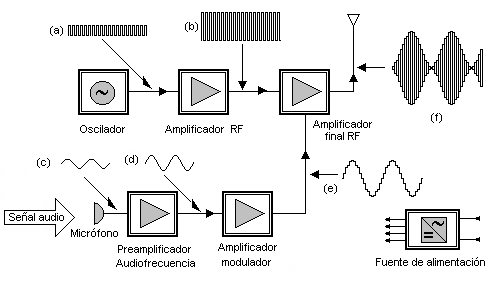
\includegraphics[width=0.65\textwidth]{figuras/Radiotransmisor.png}
\caption{Ejemplo de radiotransmisor AM}
\label{fig:radiotransmisor}
\end{figure}

Las transmisión de ondas de radio se basa en la modificación de una onda base de acuerdo a la señal que se desea transmitir. Este proceso se denomina \textbf{modulación}. Este mecanismo de modulación maximiza la cantidad de información transmitible de manera simultánea, a la vez que incrementa la robustez haciendo al sistema más resistente a ruidos, interferencias y perturbaciones. El proceso opuesto a la modulación es la llamada demodulación cuyo fin es la obtención de la señal transmitida previamente y suele ser realizada por el mismo receptor de la información.

La onda base a la que se ha hecho referencia previamente se denomina \textbf{onda portadora}. Usualmente se trata de una onda sinusoidal que puede ser modificada en alguno de sus parámetros durante el proceso de modulación previo a la transmisión \cite{Cisco:2006}.

Existen numerosas técnicas de modulación. Algunas forman parte del lenguaje popular debido a su extendido uso y otras, de un desarrollo más reciente, tienen aplicaciones más específicas.En función del parámetro sobre el que se actúe, se puede dar con diferentes tipos de modulación. A continuación se listan algunos y se comentan aquellos que tienen un uso más extendido o que tienen aplicación en el actual proyecto.

\begin{figure}[tb]
\centering
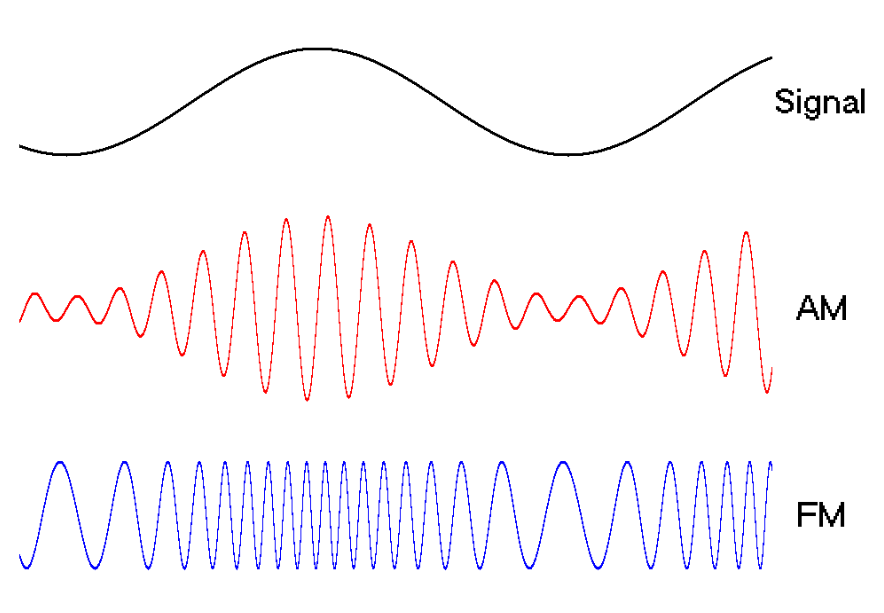
\includegraphics[width=0.55\textwidth]{figuras/Modulacion.png}
\caption{Modulación de la señal}
\label{fig:modulacion}
\end{figure}

Técnicas de modulación analógica:
\begin{itemize}
\item La \textbf{amplitud modulada}, comúnmente denominada AM, es una técnica que incide en la modificación de la amplitud de la onda portadora (figura \ref{fig:modulacion}). El resultado es una onda de igual frecuencia que la onda portadora pero que ve su amplitud variable a lo largo del tiempo en función de la señal a transmitir. Su simpleza hizo que fuera el primer método usado para tener éxito en la transmisión de audio vía telefónica.
\item La \textbf{frecuencia modulada}, o FM, se trata de una técnica de modulación focalizada en la variación de la frecuencia de la onda portadora \cite{DEI:2014} (figura \ref{fig:modulacion}). Si hablamos de aplicaciones analógicas, tras la modulación se obtiene una onda cuyo valor de la frecuencia es proporcional a la señal a transmitir. Es frecuente emplear un condensador variable denominado varactor (junto a un cristal piezoeléctrico) que varíe ligeramente la frecuencia del oscilador en función de la señal a transmitir.
\item La \textbf{modulación de fase}, también denominada PM, modifica de manera proporcional la fase de la onda portadora con la señal moduladora (figura \ref{fig:modulacionfase}). Es menos utilizada que las anteriores porque presenta ciertos problemas de ambigüedad en los extremos del rango de modulación y, especialmente, porque el coste y la complejidad de los equipos de recepción requeridos es superior.
\item Modulación de amplitud en cuadratura \cite{DEI:2014}, o QAM.
\item Modulación de doble banda lateral \cite{DEI:2014}, o DSB.
\item Modulación de banda lateral única \cite{DEI:2014}, o SSB.
\end{itemize}

\begin{figure}[tb]
\centering
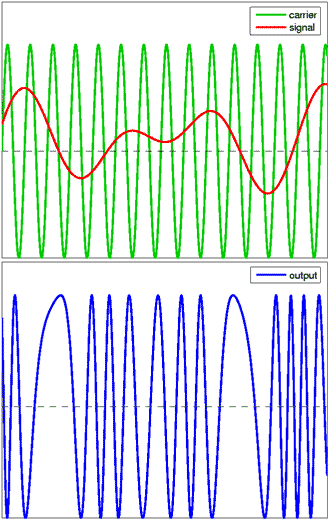
\includegraphics[width=0.55\textwidth]{figuras/ModulacionFase.png}
\caption{Modulación de fase}
\label{fig:modulacionfase}
\end{figure}

Técnicas de modulación digital:

\begin{itemize}
\item La \textbf{modulación por desplazamiento de fase}, también denominada por sus siglas en inglés PSK, consiste en la variación de la fase de la onda portadora entre una determinada variedad de valores discretos. Es, en resumen, la técnica análoga a la PM pero con la particularidad de usar una salida discreta con un número limitado de estados.
\item Modulación por desplazamiento de amplitud, o ASK.
\item Modulación por desplazamiento de frecuencia, o FSK. 
\end{itemize}

La técnica de modulación de espectro ensanchado se basa en la expansión de la señal a transmitir a lo largo de una banda muy ancha de frecuencias. Lógicamente, este método no es el más eficiente en cuanto al uso del ancho de banda pero es combinable con otros métodos que hagan uso de un ancho de banda mucho más estrecho. El receptor, al interpretar la información que llega, va a ver su ruido muy ligeramente incrementado al cohexistir con estas otras señales debido a que se dedicará a escuchas un ancho de banda muy amplio
Existen varias técnicas principales de ensanchado del espectro:

\begin{itemize}
\item El ensanchamiento de espectro por secuencia directa (figura \ref{fig:DSSS}), o DSSS, incrusta un patron de bits (pseudorruido) reduntantes entre cada uno de los bits que componen la señal a transmitir. Cuanto mayor sea este patrón de bits, más se parece la señal modulada al ruido y, consecuentemente, más interpretable como tal será por los dispositivos a los que no se dirija la información. La resistencia a interferencias es proporcional al tamaño del patron de bits.
La secuencia de bits que se utiliza para modular la señal se conoce como \textbf{secuencia de Barker} y deberá ser conocida por el receptor para poder demodular la señal y obtener la información.
Se han estandarizado dos tipos de modulación para la técnica de espectro ensanchado por secuencia directa. Una de ellas es la modulacion de fase binaria (DBPSK) y  la otra es la modulación de fase por cuadratura en offset (OQPSK). Ambas técnicas de modulación son casos específicos de la modulación por desplazamiento de fase mencionada previamente. Los módulos XBee usados en el proyecto trabajan bajo esta estandarización.
\item Ensanchamiento de espectro por salto de frecuencia, o FHSS.
\end{itemize}

\begin{figure}[tb]
\centering
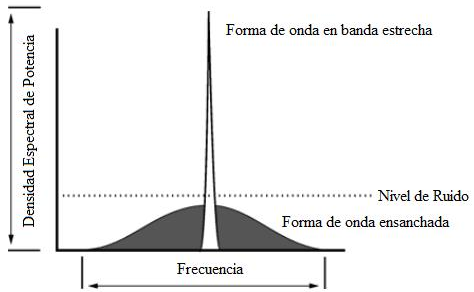
\includegraphics[width=0.55\textwidth]{figuras/DSSS.png}
\caption{Banda estrecha vs DSSS}
\label{fig:DSSS}
\end{figure}

Como sucedía en el caso de la comunicación serial, en cuanto a la transmisión vía radio frecuencia también se puede hablar de diferentes configuraciones de la línea de comunicación \cite{US_SRM:2008}. De forma análoga, uno se puede encontrar con las siguientes configuraciones:

\begin{itemize}
\item El modo de comunicación \textbf{simplex a una frecuencia}  (figura \ref{fig:simplex1}) consta de un emisor al que todos los equipos receptores estan escuchando. Es barato pero puede ocasionar problemas de interferencias o de captura de comunicación.

\begin{figure}[H]
\centering
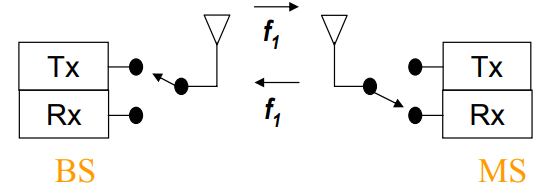
\includegraphics[width=0.55\textwidth]{figuras/RadioSimplex1.png}
\caption{Radiocomunicación simplex a una frecuencia}
\label{fig:simplex1}
\end{figure}

\item El modo \textbf{simplex a dos frecuencias} (figura \ref{fig:simplex2}) trata de evitar la interferencia entre dos dispositios emisores cercanos.

\begin{figure}[H]
\centering
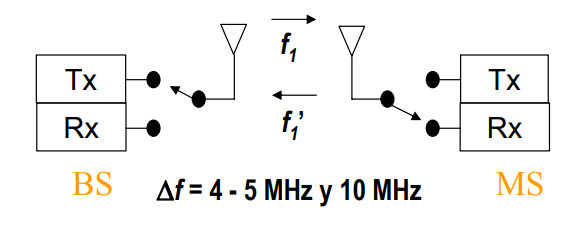
\includegraphics[width=0.55\textwidth]{figuras/RadioSimplex2.png}
\caption{Radiocomunicación simplex a dos frecuencias}
\label{fig:simplex2}
\end{figure}

\item El modo \textbf{semiduplex}  (figura \ref{fig:semiduplex}) usa un duplexor para retransmitir hacia los receptores lo que recibe de otro emisor.

\begin{figure}[H]
\centering
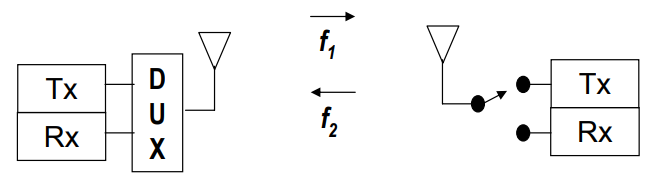
\includegraphics[width=0.55\textwidth]{figuras/RadioSemiduplex.png}
\caption{Radiocomunicación semiduplex}
\label{fig:semiduplex}
\end{figure}

\item El modo \textbf{duplex}  (figura \ref{fig:duplex}) emplea un duplexor para cada dispositivo con el fin de que todos los dispositivos funcionen de emisores y receptores con el contra de elevar el coste

\begin{figure}[H]
\centering
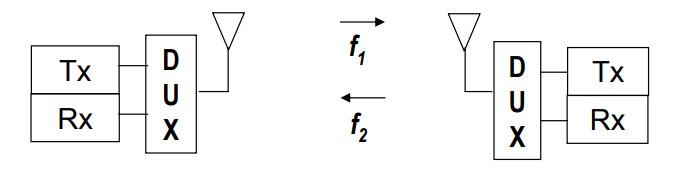
\includegraphics[width=0.55\textwidth]{figuras/RadioDuplex.png}
\caption{Radiocomunicación duplex}
\label{fig:duplex}
\end{figure}
\end{itemize}

\subsection{Problemas}

De igual manera que en cuanto a la comunicación serial el principal problema venía de la sincronización de la información, en el caso de la radiofrecuencia se puede afirmar que el principal problema proviene de las interferencias y el ruido.

Al igual que otros aspecto de la radiocomunicación como el alcance o la potencia son adaptables, existiendo un amplio rango de elección y habiendo un importante número de dispositivos muy versátiles en el mercado; el ruido electromagnético es una cuestión inevitable porque su naturaleza es igual a la de la información recibida y su existencia es inherente al entorno. Aún asi, existen formas de reducir al mínimo la influencia de este ruido.

El elemento de la antena purifica la transmisión de la señal. El uso de una alta frecuencia portadora limita su coste y tamaño manteniendo un diseño adecuado.

Varios métodos de modulación, en especial aquellos relacionados con la modulación en frecuencia, tienden a ser más inmunes a la interferencia y al ruido. Esto es debido a que un patron variado de frecuencias conocidas es más fácil de distinguir del ruido que una frecuencia permanente durante toda la transmisión. Ahí tenemos la explicación a por qué la escucha de radio FM es usualmente mas estable y de mayor calidad que la radio AM. La contra partida a esto es que la eficiencia del ancho de banda se reduce.

Por otro lado, en la etapa de modulación, se viene comprobando que, en general, conforme los procesos de transmisión y modulación se vuelven más complejos o incluyen un aumento de la velocidad de transmisión de los datos; se pierde rendimiento de la comunicación, tanto a nivel de inmunidad ante las perturbaciones, como en cuanto a la cobertura \cite{Cisco:2006}.

\subsection{Usos y aplicaciones}

La versatilidad de la radiocomunicación ha hecho que su uso se expanda en multitud de campos. A lo largo de su extensa historia, las aplicaciones han sido variadas y a continuación se listan algunas de las más representativas:

\begin{itemize}
\item Quizás la primera aplicación de las ondas de radio fue el establecimiento de redes de radioayuda que permitieran el envío de información en el conocido código morse, especialmente en el ámbito naval. Hoy en día también se implementa en la aeronavegación
\item La radio, como medio de comunicación desde que se implementara en Buenos Aires, lleva más de un siglo funcionando \cite{Zigiotto:2008}. Su influencia en el desarrollo del siglo XX es incalculable.
\item El heredero como rey de los medios de comunicación de la radio fue la televisión y también usaba esta tecnología. Hasta hace escasos años la señal de televisión se hacía llegar a las casas a través de ondas analógicas de radio que ocupaban las bandas VHF y UHF.
\item Multitud de radioaficionados y comunidades usan esta tecnología como medio de comunicación independiente a nivel local.
\item Las redes inalámbricas se han vuelto recientemente muy populares al mismo tiempo que usando, entre otros, radiofrecuencia, han ido sustituyendo a los cables. El presente proyecto viene a ser una aplicación específica de este uso.
\item Servicios de transmisión de audio y vídeo
\item Telefonía móvil
\end{itemize}